\newcommand{\bigdatachapter}{Kapitel 9. }
\chapter{Big Data und Ausblick}
\label{chapter:big-data}
\lhead{\bigdatachapter \emph{Big Data und Ausblick}}

\section{Allgemein}
Wir haben in unserem Projekt ein großes Augenmerk auf das Sammeln von Daten gelegt. Big Data ist ein Thema, auf welches man in Zeiten wie diesen, in immer mehr Bereichen des Lebens stößt. Sei es die Kontaknachverfolgung, die Digitalisierung sämtlicher gesundheitlicher und behördlicher Dokumente, oder das Sammeln von Kundendaten.

Wir und unser Projekt zählt sich eher zum Letzteren und da wir nun schon auf die Quelle der Daten, Pepper und seine Kommunikation mit den Studenten und Interessierten, sowie auf die Verarbeitung und Speicherung mit Hilfe unserer Webanwendung eingegangen sind, wollen wir nun auch noch einmal aufzeigen, was man mit diesen Informationen anfangen kann. Einen kleinen Ausschnitt haben wir schon in den Abbildungen \ref{fig:admindashboard1}, \ref{fig:admindashboard2} und \ref{fig:webappdetail} gesehen. Doch dort ist nicht mehr, als die bloße Einsicht möglich.

\section{Datenanalyse mit Python und Jupyter Notebook}
Hier kam es uns zu Gute, dass wir Teammitglieder haben, welche sich auch mit Jupyter Notebooks sehr gut auskennen. So ist es passiert, dass wir eine Client Klasse in Python geschrieben haben, welche es uns ermöglicht, durch bloße Eingabe des API Keys, auf Daten in unserer Webanwendung zuzugreifen. Hierfür wird der Endpunkt \verb|/docker-hbv-kms-http/api/v1/sql| angesprochen, an welchen wir unsere SQL Abfragen schicken können und die Ergebnisse als Antwort von unserer Webanwendung zurück bekommen.

Die Client Klasse sorgt automatisch dafür, dass die Anfragen entsrechend formatiert und abgeschickt werden, sowie Fehler ohne Probleme behandelt und mitgeteilt werden. Somit bekommt der Nutzer in seinem Jupyter Notebook mitgeteilt, sofern er einen Fehler in seiner SQL Syntax hat, da wir auch diese Informationen von unserem Server an den Benutzer übermitteln. Nachfolgend ist ein solches Beispiel vorgeführt:\\

\begin{lstlisting}
    [ IN ]  client = Client(API_KEY, sandbox=False)
    [ OUT ] {'message': 'Connected!'}
    [ IN ]  client.sql_query("select * from users")
    [ OUT ] Exception: 400-Invalid SQL command!
\end{lstlisting}

Wer sich an Abschnitt \ref{sec:api-sql-query} erinnert wird bemerken, dass die Tabelle \verb|users| nicht über diesen Endpunkt ansprechbar ist.

Der Parameter \verb|sandbox|, welcher im Konstruktor der Client Klasse verarbeitet wird, gibt an, ob man sich mit der lokalen Instanz der Webanwendung, oder mit der in der Produktivumgebung verbinden möchte.

Hat man nun die Client Klasse instantiiert, ist es mit ihr möglich eine Vielzahl von SQL Abfragen durchzuführen, um an verschiedene von Pepper gespeicherte Konversationsdaten zu gelangen.

Mit Hilfe der Bibliotheken Pandas, Matplotlib und weiteren, haben wir innerhalb dieses Notebooks verschiedene Visualisierungen angefertigt. Hierbei ist zu beachten, dass all diese Daten mit Hilfe des Skriptes aus Abschnitt \ref{sec:dummy-data} generiert worden sind.\\

\begin{figure}[H]
    \centering
    \begin{minipage}[b]{0.49\textwidth}
        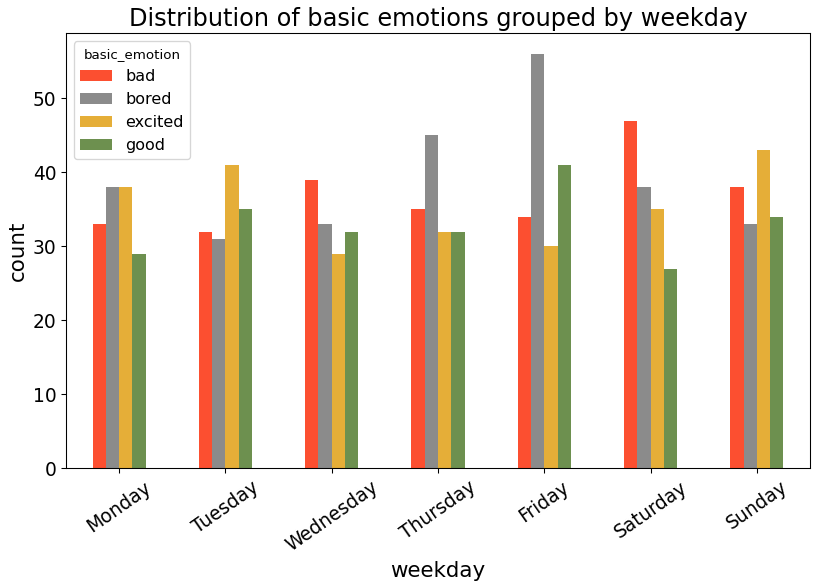
\includegraphics[width=\textwidth]{Figures/analysis/emotionwd.png}
        \caption{Diagramm: Emotion je Wochentag}
        \label{fig:emotionwd}
    \end{minipage}
    \hfill
    \begin{minipage}[b]{0.49\textwidth}
        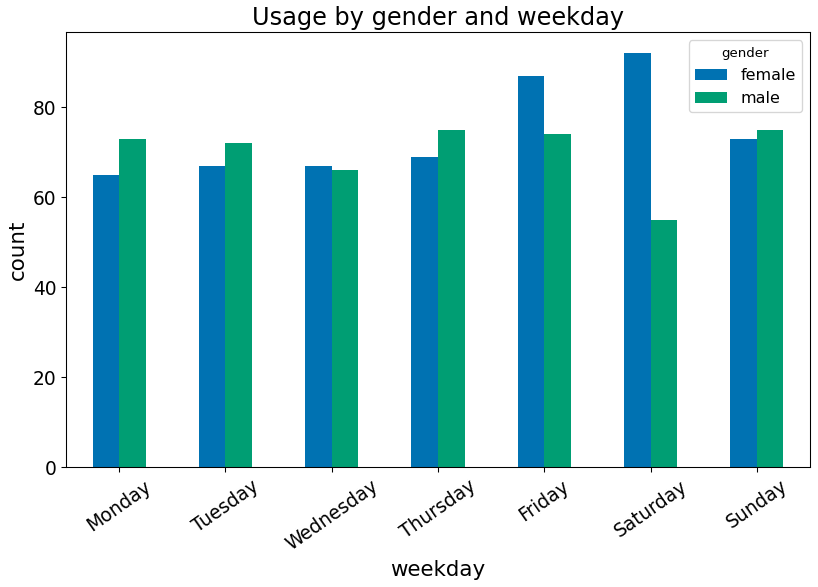
\includegraphics[width=\textwidth]{Figures/analysis/genderwd.png}
        \caption{Diagramm: Geschlecht je Wochentag}
        \label{fig:genderwd}
    \end{minipage}
\end{figure}

\begin{figure}[H]
    \centering
    \begin{minipage}[b]{0.49\textwidth}
        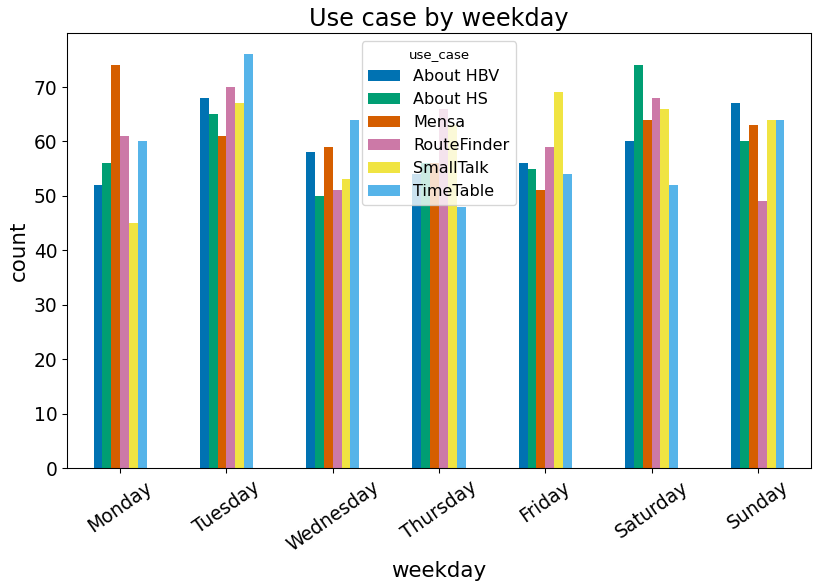
\includegraphics[width=\textwidth]{Figures/analysis/usecasewd.png}
        \caption{Diagramm: UseCase je Wochentag}
        \label{fig:usecasewd}
    \end{minipage}
    \hfill
    \begin{minipage}[b]{0.49\textwidth}
        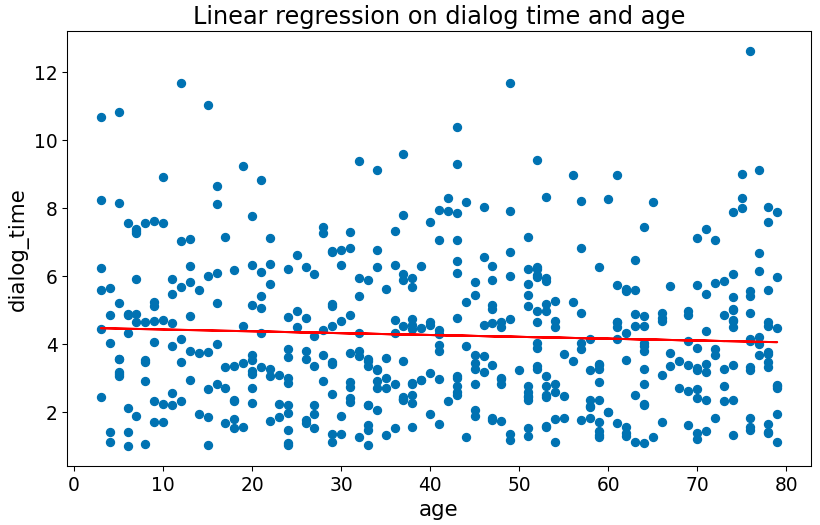
\includegraphics[width=\textwidth]{Figures/analysis/linreg.png}
        \caption{Diagramm: Lineare Regression zwischen Dialog Zeit und Alter}
        \label{fig:linreg}
    \end{minipage}
\end{figure}

Die Abbildungen \ref{fig:emotionwd} ff. geben einen kleinen Vorgeschmack auf die Möglichkeiten der Analyse der von Pepper sammelbaren Daten. in dem Notebook sind weitere Diagramme zu finden, auch ein simples RNN wurde konstruiert, mit welchem wir das Alter anhand der zur Verfügung stehenden Parameter bestimmen wollten. Jedoch es nicht verwunderlich, dass wir bei einer Genauigkeit von 50\% liegen, da diese Daten von uns generiert worden sind.

Diese Schnittstelle zu unserem Webserver ermlglicht es dem Anwender, einen genaueren Einblick in die Daten zubekommen. Zusätzlich zu diesem Notebook, haben wir ein Skript erstellt, welches die Daten aus der Datenbank abruft und die Visualisierungen als PDF Datei speichert. Dies ist in Verbindung mit einem Cronjob, einem wiederkehrenden Prozess sehr nützlich, denn so können wir, aber auch andere, die diese Art der Anwendung nutzen wollen, sich in regelmäßigen Abständen Berichte generieren lassen, welche einen tieferen Einblick in die Daten bieten.

Durch die Anbindung von Pepper an unsere Webanwendung ist es möglich, sämtliche Informationen, während einer Konversation zu speichern und nachzuvollziehen. Hiermit können Unternehmen herusfinden, was ihre Kunden bewegt und in welchen Bereichen man noch an seinem Geschäftsmodell arbeiten muss. Es wäre Denkbar, mehrere Pepper, welche den selben Datensammlungsablauf haben, an verschiedene Unternehmen zu vermieten, womit man als Vermiter ein großes Kontingent an Informationen zu verschiedenen Branchen sammeln und auswerten kann.\\

\subsection{Mögliche Erweiterungen}

\subsubsection{Google Dialogflow}

Dialog Flow, ist eine von dem Konzern Google betriebene Plattform, welche das verarbeiten und verstehen von menschlicher Sprache ermöglicht. Sie bietet den Vorteil, dass die Verarbeitung der Sprache nicht mehr auf dem eigenen System stattfinden, sondern an einen von Google bereitgestellten Server gesendet wird. Dieser verarbeitet die Daten und sendet sie anschließend wieder zurück. Dialog Flow hat dabei den Vorteil, dass sich die Interaktion der Dialoge dynamisch auf der von Google erstellten Browser-Plattform bearbeiten lassen. Eine Implementierung in das Pepper System, könnte so das produktive Arbeiten stark verbessern. Es ist außerdem möglich Lernraten zu definieren, durch welche Pepper, ohne das erneute Aufspielen einer Applikation dazu lernen könnte. Pepper wäre mit einer solchen Architektur in der Lage, selbst und dynamisch dazuzulernen und seine Interaktion und das Verstehen von Wörtern und Sprache ständig weiter zu optimieren. Wir haben für diese Funktionalität ein grafisches Konzept erstellt, welches den Ablauf dieser theoretischen Funktionalität verdeutlichen soll:



Obwohl es eine von SoftBanks-Robotik offiziell bereitgestellte Schnittstelle für eine Anbindung an die Google-Dialogflow Plattform gibt, haben wir uns nicht nur aus zeitlichen Gründen gegen die Entwicklung einer solchen Funktionalität entschieden. Dabei gab es für uns zwei entscheidende Faktoren. Erstens empfinden wir es als äußerst unpassend, unser bereits entwickeltes System, welches dem Administrator den Vorteil bietet, die gesammelten Daten selbst zu besitzen, mit einer Anwendung zu verknüpfen, durch welche diese an einen Großkonzern weitergegeben werden. Das würde für uns bedeuten, dass wir einen unserer bedeutendsten Schwerpunkte dieser Arbeit verlieren, und zwar das ermöglichen gesammelte Daten selber zu verwalten und beliebig in eigene Dateiformate zu konvertieren und weiterzuverarbeiten. Außerdem ist es so, dass Google die Dialogflow Plattform nur für zahlende Kunden in Form eines Abo-Modells anbietet, wobei hier Mikrobeträge pro Request an die Plattform bezahlt werden müssen. Es wäre also alleine schon ein Kostenfaktor, eine Anwendung, während des Entwicklungsprozesses mit diesem System zu testen. Trotzdem möchten wir der Vollständigkeitshalber auf die Möglichkeit der Anbindung an Google Dialog hinweisen, auch wenn sie sich nicht mit den Ethischen-Vorstellungen unserer Softwareanwendung vereinbaren lassen.

\subsubsection{Dynamisches Bewegen im Raum}

Es ist möglich, Pepper das Bewegen in einem Raum beizubringen. Dies würde den Roboter für den Benutzer noch menschlicher erscheinen lassen, da es den Roboter um die Eigenschaft der Proxemik erweitern würde. Außerdem könnte Pepper so Routen ablaufen, um evtl. noch mehr Benutzer für die Interaktion zu finden und diese auf sich aufmerksam zu machen. Auch das automatische Ansteuern einer Ladestation wäre durch diese Funktion möglich, wodurch Pepper autonomer und noch unabhängiger von der Betreuung eines Menschen während seiner Arbeit wird.

\subsubsection{Sozialmedia-Bot}

Während der Arbeit an und mit Pepper fiel uns vor allem das außerordentliche Interesse auf, welches bei Passanten zu beobachten war. Es kam zudem des Öfteren vor, dass der Roboter gefilmt wurde oder man uns fragte, ob es möglich sei ein “Selfi” mit dem Roboter zu machen. Die von Pepper ausgelöste Neugier bei Menschen hat, inspirierte uns zu dem Konzept, den Roboter selbst als Social-Media-Marketing Instrument einzusetzen.
Ein solcher Anwendungsfall wäre durch die Implementierung eines oder mehrerer Bots (automatisierter Accounts) in die Architektur unserer Anwendung umsetzbar. Es wäre somit möglich, dass der Roboter bewusst Benutzer dazu auffordert, mit ihnen zu interagieren und ein Selbstporträt zu machen. Im Anschluss daran könnte der Bot mit einem zufällig gewählten Kommentar auf das veröffentlichte Bild regieren, wenn er erkennt, dass er auf diesem verlinkt wurde. Außerdem könnte der Bot selbstständig Veröffentlichungen aus den von ihm gesammelten Daten erstellen, in welchem er diese visuell darstellt und interpretiert. Pepper könnte so für seinen Besitzer einen positives Marketingeffekt erzielen.

\subsection{Weitere potenzielle Einsatzbereiche}

Wir haben während der Entwicklung mit Pepper, noch eine Reihe weitere Anwendungsfälle für unsere Software-Architektur definiert. Drei dieser Einsatzbereiche haben wir im Folgendem aufgelistet.

\subsubsection{Gastronomie}

Es könnte ein System wie das aus dem Bachelor-Projekt mit Pepper als Möglichkeit zum Daten sammeln für die Gastronomie interessant sein. Pepper könnte Kunden zu ihrer Zufriedenheit befragen, Bestellungen aufnehmen oder über das Hygienekonzept informieren. Die dabei gesammelten Daten lassen sich flexibel analysieren, um ein genaueres Bild über die Kunden zu ermitteln und dies für potenzielle Optimierung von Geschäftsprozessen zu einzusetzen.

\subsubsection{Krankenhäuser und Pflegeeinrichtungen}

Pepper, könnte viele zwischenmenschliche Aufgaben in einem Pflegeheim erfüllen. Zudem wäre es mit der von uns entwickelten Software-Architektur möglich, den gesundheitlichen Zustand und das generelle Wohlbefinden eines Bewohners einzuordnen und anschließend zu auf einem Server zu dokumentieren. Der Roboter könnte die Menschen in einer Einrichtung dabei spielerisch im Alltag unterstützen, während er Daten über die physische, sowie psychische Befindlichkeit sammelt. Wie die Daten können anschließend von Mitarbeitern des Pflegeheims ausgewertet werden.

\subsubsection{Kaufhäuser}

Große Einkaufszentren könnten die Anwendung ähnlich nutzen, wie wir es in unserem Entwurf für die Hochschule getan haben. Der Roboter würde Wegrouten beschreiben oder über das Kaufhaus informieren. Zusätzlich wäre es hier auch von Nutzen, den Roboter um ein Konzept wie in \ref{sec:Sozialmedia-Bot} beschrieben zu erweitern. Außerdem könnte Pepper so programmiert werden, dass er Anfragen zu spezifischen Produkten entgegennimmt, um dem Benutzer die entsprechenden Geschäfte zu nennen, in welchen es dieses zu erwerben gibt.
